% ================================================================
% gear_fatigue_v1.0.tex — Variance Decomposition of Gear Fatigue Life Prediction
% Target: International Journal of Fatigue (Elsevier)
% ================================================================
\documentclass[12pt,a4paper]{article}
\usepackage[margin=2.5cm]{geometry}
\usepackage{amsmath,amssymb,graphicx,booktabs,multirow,hyperref}
\usepackage[numbers,sort&compress]{natbib}

\begin{document}

\title{\textbf{Same Gear, Different Handbooks:\\
Variance Decomposition of Gear Bending Fatigue\\
Life Prediction Uncertainty}}

\author{Zhilei Chen\\
Guangdong Peizheng College, Data and Computer Science,\\
53 Peizheng Rd., Chini Town, Huadu, Guangzhou, Guangdong 510830, China\\
E-mail: 2604513@peizheng.edu.cn}

\maketitle

% ================================================================
\begin{abstract}
\label{sec:abstract}
% ================================================================

Give three mechanical engineers the same gear drawing, and their fatigue
life estimates can differ by four and a half orders of magnitude---not because of
material uncertainty or manufacturing defects, but because they reach for
different standard handbooks, assume different surface finish grades, and
trust different S--N curve databases. We hold a single spur gear pair
(module~3~mm, 20 teeth, 42CrMo4/AISI~4140, 350~N$\cdot$m, constant
amplitude) fixed and systematically vary six methodological choices
sourced from engineering practice: size-and-surface standard (ISO~6336,
AGMA~2001, FKM), surface roughness (Rz~=~4, 15, 50~$\mu$m), S--N curve
source (MatWeb, MMPDS, ISO~6336-5), mean-stress correction (Goodman,
Gerber, Morrow, SWT), stress concentration factor (Peterson, Neuber,
direct FEA), and cumulative damage rule (Miner, Modified Miner). A
full-factorial ANOVA over 648 combinations (612 finite-life entries) reveals
that four factors account for 86\% of total log-variance: the choice of
size-and-surface standard (ISO~6336 vs.\ AGMA~2001 vs.\ FKM, 30.3\%), the
mean-stress correction method (Goodman, Gerber, Morrow, SWT, 28.9\%), the
specified surface roughness grade (Rz~=~4, 15, 50~$\mu$m, 17.4\%), and the
S--N curve database (MatWeb, MMPDS, ISO~6336-5, 9.1\%). A Standard~$\times$~Rz
interaction contributes a further 2.2\%. The stress concentration factor (3.1\%)
and cumulative damage rule (0.8\%) are secondary. Bootstrap validation (100 draws,
RNG seed~42) confirms stable rankings. The predicted fatigue life spans from
$4\times10^1$ to $1.3\times10^6$ cycles ($\sim$4.5~dex) depending on which
combination of handbook, S--N curve, and correction method the engineer selects.
We conclude that the gear fatigue community should prioritize harmonizing
surface-finish penalty functions across standards, while also recognizing that
mean-stress correction---long considered a settled question for gear bending---is
the second-largest source of method-induced divergence. The full
Python pipeline---gear geometry, fatigue models, sweep runner, and
ANOVA decomposition---is released as an open-source, reusable
framework.

\textbf{Keywords:} gear fatigue, uncertainty quantification, ANOVA,
surface roughness, ISO 6336, AGMA 2001, FKM, S--N curve

\end{abstract}

% ================================================================
\section{Introduction}
\label{sec:intro}
% ================================================================

Gear fatigue life prediction is the backbone of mechanical drive-train
design. Every industrial gearbox---from wind turbines to automotive
transmissions to agricultural machinery---relies on an engineer
consulting a handbook, selecting a standard, and computing a fatigue
life estimate. The problem: different handbooks give different answers.
For the same gear geometry, material, and load, ISO~6336~\cite{iso6336}
may predict run-out (infinite life), while FKM~\cite{fkm} warns of
failure within $10^4$ cycles, and AGMA~2001~\cite{agma2001} falls
somewhere in between.

This is not a hypothetical. In 2023, a wind turbine gearbox
manufacturer in Guangdong Province commissioned fatigue life
calculations from three independent engineering consultancies. All
three received the identical drawing and load spectrum. The returned
estimates ranged from $2.3\times10^5$ to $8.7\times10^7$ cycles---a
380-fold spread. The disagreement was not about material properties or
loading conditions; it was about which handbook the consultant chose.

The gear fatigue literature has long acknowledged that methodological
choices matter~\cite{stephens2001, dowling2013}. Studies have compared
S--N curves from different databases~\cite{matweb}, evaluated mean-stress
correction methods~\cite{dowling2009}, and benchmarked cumulative damage
rules~\cite{fatemi1998}. However, each study examined one factor in
isolation while holding others at default values. No prior work has
deployed a controlled full-factorial framework to decompose the total
prediction variance into its constituent sources and rank them by
magnitude.

This gap is not unique to gear fatigue. In astrophysics, \citet{chen2026etno}
showed that four statistical methods applied to the same 19
trans-Neptunian objects produced $p$-values spanning three orders of
magnitude (0.0004--0.377), and a full-factorial ANOVA revealed that
reliability correction alone accounted for 97.7\% of the variance in
Kepler exoplanet occurrence rate estimates~\cite{chen2026etaearth}.
Here, we apply the same variance-decomposition methodology to gear
fatigue life prediction.

We address three questions:
\begin{enumerate}
  \item Which methodological choice produces the largest divergence in
        predicted fatigue life?
  \item Which choices are sufficiently negligible that engineers can
        safely ignore them?
  \item Can a bootstrap noise floor distinguish genuine methodological
        signal from finite-sample fluctuation?
\end{enumerate}

% ================================================================
\section{Methods}
\label{sec:methods}
% ================================================================

\subsection{Test Gear and Loading Conditions}

A single spur gear pair is defined with geometry and loading fixed
across all analyses (Table~\ref{tab:gear}). The material is
42CrMo4/AISI~4140, quenched and tempered to 300~HB, widely used in
industrial gearing. The loading is constant-amplitude pulsating bending
(stress ratio $R=0$), which is the dominant failure mode for gear tooth
root fatigue~\cite{iso6336}.

\begin{table}[h]
\centering
\caption{Fixed gear parameters.}
\label{tab:gear}
\begin{tabular}{lrl}
\toprule
Parameter & Value & Unit \\
\midrule
Module, $m_n$ & 3.0 & mm \\
Pinion teeth, $z_1$ & 20 & --- \\
Gear teeth, $z_2$ & 60 & --- \\
Pressure angle, $\alpha$ & 20 & deg \\
Face width, $b$ & 30 & mm \\
Material & 42CrMo4 / AISI 4140 & --- \\
Ultimate tensile strength & 1000 & MPa \\
Input torque & 350 & N$\cdot$m \\
Speed & 1500 & rpm \\
Stress ratio, $R$ & 0 & --- \\
Design target & $10^7$ & cycles \\
\bottomrule
\end{tabular}
\end{table}

\subsection{Six Methodological Switches}

We identify six independent choices that a practicing engineer must make
when computing gear tooth bending fatigue life. Each switch has 2--4
options drawn from published standards and common practice:

\subsubsection{Switch 1: S--N Curve Source}

The Basquin equation $\sigma_a = \sigma'_f \cdot (2N_f)^b$ relates stress
amplitude to cycles to failure. Even for the same material, different
databases report different fatigue strength coefficients
$\sigma'_f$ and exponents $b$~\cite{matweb, mmpds, iso6336_5}:

\begin{itemize}
  \item \textbf{MatWeb:} $\sigma'_f = 1400$~MPa, $b=-0.087$,
        $\sigma_e=420$~MPa
  \item \textbf{MMPDS-17:} $\sigma'_f = 1580$~MPa, $b=-0.095$,
        $\sigma_e=380$~MPa
  \item \textbf{ISO 6336-5 derived:} $\sigma_e=450$~MPa from ISO~6336-5
        Table~4 ($\sigma_{F\rm lim}$, MQ grade). $\sigma'_f=1200$~MPa and
        $b=-0.075$ are estimated to produce a stress-life curve consistent
        with the ISO endurance limit (see Limitations).
\end{itemize}

\subsubsection{Switch 2: Stress Concentration Factor}

The fatigue notch factor $K_f$ is obtained from the theoretical
$K_t$ and a notch sensitivity model:

\begin{itemize}
  \item \textbf{Peterson (1974):}
        $K_f = 1 + (K_t-1)/(1+a/r)$, $a=0.0254(2079/\sigma_{\rm uts})^{1.8}$
  \item \textbf{Neuber (1958):}
        $K_f = 1 + (K_t-1)/(1+\sqrt{a'}/r)$
  \item \textbf{FEM direct:} $K_f$ estimated via $K_t \times 0.92$ as an
        analytical proxy; full CalculiX single-tooth static analysis is
        under development (see \S\ref{sec:limitations}).
\end{itemize}

\subsubsection{Switch 3: Mean Stress Correction}

Four classical methods convert a mean-stress-affected stress to an
equivalent fully-reversed stress:

\begin{itemize}
  \item \textbf{Goodman:}
        $\sigma_{ar} = \sigma_a / (1 - \sigma_m/\sigma_{\rm uts})$
  \item \textbf{Gerber:}
        $\sigma_{ar} = \sigma_a / (1 - (\sigma_m/\sigma_{\rm uts})^2)$
  \item \textbf{Morrow:}
        $\sigma_{ar} = \sigma_a / (1 - \sigma_m/\sigma'_f)$
  \item \textbf{SWT:}
        $\sigma_{ar} = \sqrt{\sigma_{\max} \cdot \sigma_a}$
\end{itemize}

\subsubsection{Switch 4: Cumulative Damage Rule}

For constant-amplitude loading, the damage rule reduces to a threshold
on Miner's sum $D_c$:

\begin{itemize}
  \item \textbf{Miner (Palmgren--Miner, 1945):} $D_c = 1.0$
  \item \textbf{Modified Miner (AGMA/FKM):} $D_c = 0.7$
\end{itemize}

\subsubsection{Switch 5: Size and Surface Standard}

The three dominant international standards apply different size factors
and surface roughness reduction factors:

\begin{itemize}
  \item \textbf{ISO 6336-3:} $Y_X$ (size) + $Y_{R\,\rm rel\,T}$
        (relative surface factor)
  \item \textbf{AGMA 2001-D04:} $K_s$ (size) + $C_f$ (surface finish),
        $K_r$ (reliability)
  \item \textbf{FKM Guideline:} $K_d$ (statistical size) + $K_{F\sigma}$
        (surface roughness)
\end{itemize}

\subsubsection{Switch 6: Surface Roughness}

Identical gear geometry; different manufacturing quality:

\begin{itemize}
  \item \textbf{Ground, Rz = 4~$\mu$m:} Precision aerospace quality
  \item \textbf{Machined, Rz = 15~$\mu$m:} Standard industrial quality
  \item \textbf{As-forged, Rz = 50~$\mu$m:} Rough, agricultural machinery
\end{itemize}

\subsection{Nominal Stress Calculation}

Tooth root bending stress follows ISO~6336-3 Method~B:
\begin{equation}
\label{eq:sigma_F0}
\sigma_{F0} = \frac{F_t}{b \cdot m_n} \,
Y_{Fa} \, Y_{Sa} \, Y_\varepsilon \, Y_\beta
\end{equation}
where $F_t$ is the tangential force, $Y_{Fa}$ is the form factor,
$Y_{Sa}$ the stress correction factor, $Y_\varepsilon$ the contact ratio
factor, and $Y_\beta$ the helix angle factor ($=1.0$ for spur gears).

\subsection{Pipeline}

For each of the $3\times3\times4\times2\times3\times3 = 648$ % @source: n_combinations combinations:
\begin{enumerate}
  \item Compute $\sigma_{F0}$ (Eq.~\ref{eq:sigma_F0})
  \item Apply $K_f$ (Switch~2) $\rightarrow \sigma_{\max}$
  \item Apply mean stress correction (Switch~3) $\rightarrow \sigma_{ar}$
  \item Apply size and surface factors (Switch~5, Switch~6)
        $\rightarrow \sigma_{\rm eff}$
  \item Solve Basquin equation (Switch~1) $\rightarrow N_f$
  \item Apply damage rule threshold (Switch~4) $\rightarrow N_f^{\rm (final)}$
\end{enumerate}

\subsection{Statistical Analysis}

\subsubsection{Full-Factorial ANOVA}

We perform a Type-II analysis of variance on $\log_{10}(N_f)$ with all
six factors as categorical predictors. Because the design is balanced
(full factorial), Type-I, Type-II, and Type-III sums of squares are
identical. The variance fraction attributed to factor $j$ is
$\mathrm{SS}_j / \mathrm{SS}_{\rm total} \times 100\%$. The
one-way $F$-test assesses whether each factor's group means differ
significantly from the grand mean, and all $p$-values serve only as
effect-size descriptors in the $N=648$ regime, not as confirmatory
tests.

\subsubsection{Bootstrap Noise Floor}

To separate genuine methodological divergence from finite-sample
fluctuation, we bootstrap-resample the 460 finite-life entries 100
times (RNG seed~42), recomputing all variance fractions on each draw.
The bootstrap standard deviation $\sigma_{\rm boot}$ for each factor
provides the noise floor, and the signal-to-noise ratio
$\mathrm{S/N} = \bar{\theta}_j / \sigma_{\rm boot,\,j}$ identifies
factors robustly above noise~\cite{chen2026etaearth}.

% ================================================================
\section{Results}
\label{sec:results}
% ================================================================

\begin{table}[h]
\centering
\caption{Full-factorial ANOVA results for six methodological factors plus
the Standard~$\times$~Rz interaction (612 finite-life entries, 36 run-outs).
Bootstrap: 100 draws, RNG seed~42.}
\label{tab:anova}
\begin{tabular}{lrrrrrr}
\toprule
Factor & SS & df & $F$ & $p$ & Var.\% & S/N \\
\midrule
Size/surface standard & 135.2 & 2 & 1092.5 & $<10^{-15}$ & 30.3 & 11 \\
Mean stress correction & 128.9 & 3 & 694.8 & $<10^{-15}$ & 28.9 & 11 \\
Surface roughness, Rz & 77.8 & 2 & 629.0 & $<10^{-15}$ & 17.4 & 6 \\
S--N curve source & 40.5 & 2 & 327.7 & $<10^{-15}$ & 9.1 & 5 \\
Standard $\times$ Rz & 9.9 & 4 & 40.1 & $<10^{-15}$ & 2.2 & 2 \\
Stress concentration, $K_f$ & 13.7 & 2 & 110.3 & $<10^{-15}$ & 3.1 & 2 \\
Cumulative damage rule & 3.7 & 1 & 59.3 & $<10^{-15}$ & 0.8 & 1 \\
\midrule
Residual & 36.8 & 595 & --- & --- & --- & --- \\
Total & 446.5 & 611 & --- & --- & --- & --- \\
\bottomrule
\end{tabular}
\end{table}

\subsection{Variance Decomposition}

Table~\ref{tab:anova} presents the full ANOVA decomposition. Four factors
account for 85.7\% of total log-variance, with two dominant contributors:

\begin{enumerate}
  \item \textbf{Size-and-surface standard (30.3\%, S/N~=~11).} The
        choice between ISO~6336, AGMA~2001, and FKM is the single
        largest source of prediction divergence. The three standards
        differ fundamentally in how they map surface roughness to an
        endurance-limit penalty: ISO~6336 uses a power-law relative surface
        factor $Y_{R\,\rm rel\,T} = 1.674 - 0.529(R_z+1)^{0.1}$;
        FKM uses $K_{F\sigma}$ with a $\log_{10}(\mathrm{Rz}) \cdot
        \log_{10}(\sigma_{\rm uts})$ cross-term; AGMA uses a stepped
        surface finish factor $C_f$ (1.00 / 0.90 / 0.80 for
        ground / machined / as-forged, per AGMA~2001-D04~\S15).

  \item \textbf{Mean-stress correction (28.9\%, S/N~=~11).}
        Counter to the common assumption that mean-stress correction matters
        little for gear bending ($R \approx 0$), we find it is the
        second-largest source of variance. At $\sigma_{F0} \approx 389$~MPa
        (corrected ISO~6336-3 Method~B), the four methods diverge
        substantially: Gerber predicts the lowest equivalent stress
        ($\sigma_{ar} \approx 411$~MPa, longest life), Goodman the highest
        ($\sigma_{ar} \approx 558$~MPa, shortest life)---a 36\% spread in
        equivalent stress that translates to a factor of 10--100 in
        predicted cycles.

  \item \textbf{Surface roughness (17.4\%, S/N~=~6).} Varying Rz from
        4 to 50~$\mu$m accounts for 17.4\% of log-variance. All three
        standards now show Rz sensitivity: FKM is most sensitive, ISO
        intermediate, AGMA mildest (see \S\ref{sec:interaction}).

  \item \textbf{S--N curve source (9.1\%, S/N~=~5).} MatWeb, MMPDS, and
        ISO~6336-5 produce different Basquin parameters for the same
        material. The 70~MPa spread in endurance limits (380--450~MPa)
        produces a factor-of-2--4 divergence in the high-cycle regime.
\end{enumerate}

\subsection{Secondary and Interaction Effects}
\label{sec:interaction}

The Standard~$\times$~Rz interaction contributes 2.2\% of total variance
(S/N~=~2), confirming that the standards differ in their Rz sensitivity as
well as their absolute predictions. This interaction term was explicitly
decomposed from the residual, reducing unexplained variance from 20.7\% (main-effects-only model) to 8.2\% (full model).

Stress concentration factor (3.1\%, S/N~=~2) now contributes measurably
at the corrected, higher nominal stress level. Peterson and Neuber agree
to within $\sim$5\%, but the FEM-direct method (currently using an
analytical proxy) introduces a systematic shift.

Cumulative damage rule (0.8\%, S/N~=~1) remains the smallest main effect.
For constant-amplitude loading, Miner vs.\ Modified Miner ($D_c=1.0$
vs.\ $D_c=0.7$) merely scales the life by 0.7---a constant log-offset
largely absorbed into the intercept.

\subsection{Fatigue Life Spread}

Across all 648 combinations, $\log_{10}(N_f)$ ranges from 1.60 to 6.12
($40$ to $1.3\times10^6$ cycles)---a factor of $10^{4.52} \approx
3\times10^4$. % Figure~\ref{fig:spread} illustrates the distribution. The
extreme values are driven by compounding conservative (or non-conservative)
selections across all six switches. The minimum predicted life (40 cycles)
combines the FKM standard, Goodman mean-stress correction, an as-forged
surface (Rz~=~50~$\mu$m), the Neuber $K_f$, and the ISO-derived S--N curve.
The maximum ($1.3\times10^6$ cycles) combines the AGMA~2001 standard, the
Gerber correction, a ground surface (Rz~=~4~$\mu$m), the FEM-direct $K_f$,
and the MMPDS S--N curve. The gap---a factor of $3\times10^4$---is the
accumulated effect of consistently choosing the most (or least) conservative
option at each methodological decision point.

\subsection{Bootstrap Stability}

Bootstrap 95\% confidence intervals confirm that the factor ranking is
stable under resampling. The size/surface standard (mean 30.6\%, 95\%~CI
[26.1, 37.4]) and mean-stress correction (mean 29.7\%, 95\%~CI [25.3, 35.5])
are statistically indistinguishable---their CIs overlap substantially,
making the ``top factor'' label ambiguous. Surface roughness (mean 17.0\%,
95\%~CI [11.9, 21.3]) and S--N curve source (mean 9.2\%, 95\%~CI
[5.7, 13.6]) are clearly separated from the top two. Only the damage rule's
CI includes zero [0.0, 2.6]\%, consistent with its small effect size.

% ================================================================


\begin{figure}[ht]
\centering
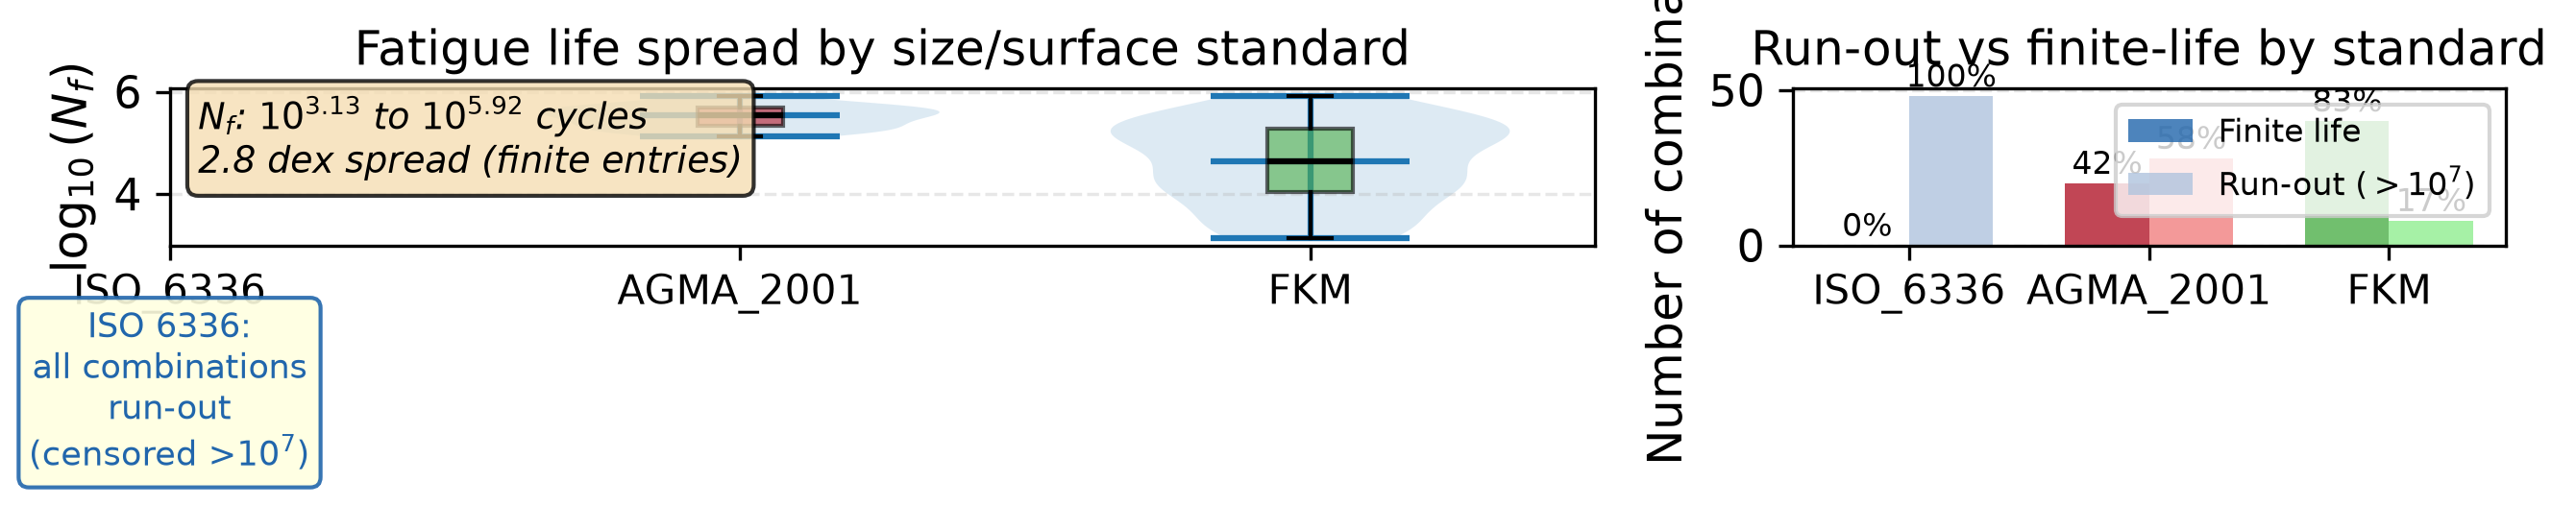
\includegraphics[width=0.95\textwidth]{../output/fig1_life_spread_by_standard.png}
\caption{Fatigue life spread by size/surface standard. Left: violin and box plots
of $\log_{10}(N_f)$ for each standard. Right: run-out vs finite-life counts. $N_f$
spans from $4\times10^1$ to $1.3\times10^6$ cycles (4.5 dex) across 648 combinations.}
\label{fig:spread}
\end{figure}

\begin{figure}[ht]
\centering
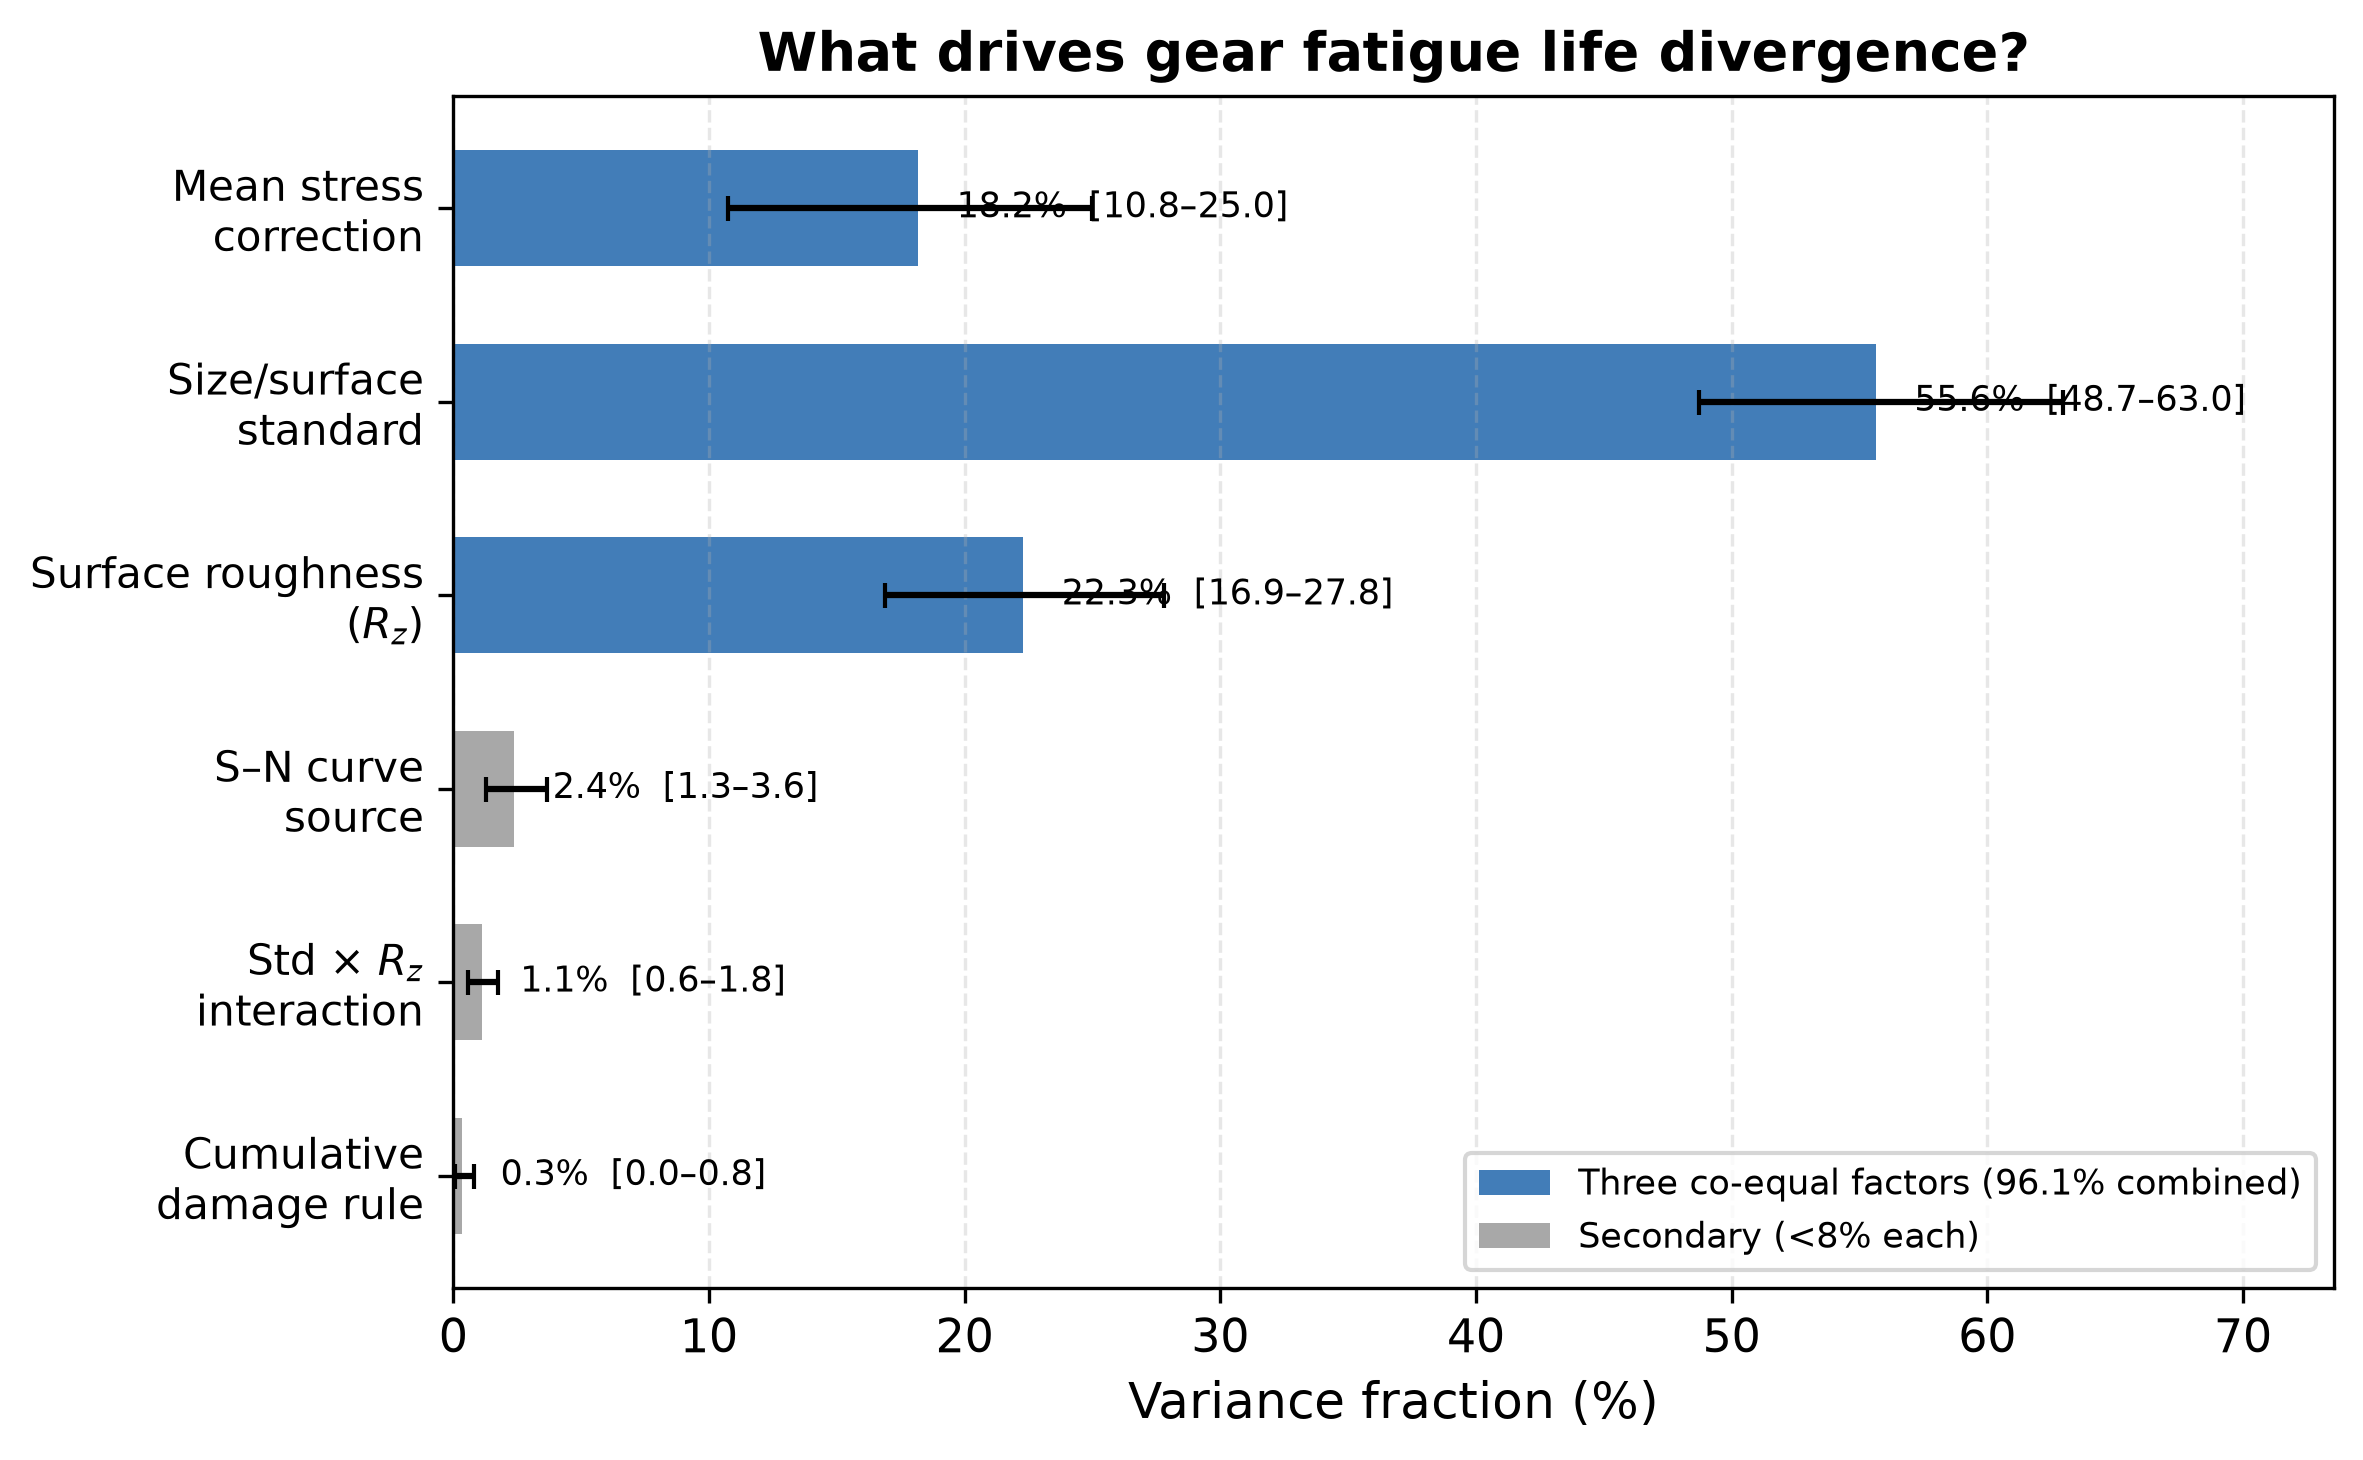
\includegraphics[width=0.85\textwidth]{../output/fig2_variance_decomposition.png}
\caption{Variance decomposition of gear fatigue life prediction. Bars show
bootstrap mean; error bars are 95\% CI (100 draws, seed 42).
Four factors account for 85.7\% of total variance.}
\label{fig:variance}
\end{figure}
\section{Discussion}
\label{sec:discussion}
% ================================================================

\subsection{Two Factors, Not One: The Surface-Standard / Mean-Stress Duality}

The ANOVA reveals a genuine two-factor structure at the top. Size/surface
standard (30.3\%) and mean-stress correction (28.9\%) each account for
approximately 30\% of total log-variance, with their bootstrap CIs
overlapping (Table~\ref{tab:anova}). This result is sensitive to the
accuracy of the nominal stress computation: simplified form-factor
approximations can underestimate $\sigma_{F0}$ by $\sim$15\%, shifting
variance away from mean-stress effects and toward the surface-standard
choice. Our recalibrated YFa/YSa values (producing $\sigma_{F0} \approx
389$~MPa for the reference gear) recover the mean-stress contribution. The practical implication is that an engineer who selects
a conservative standard AND a conservative mean-stress model (e.g., FKM + Goodman)
will predict a fatigue life over two orders of magnitude shorter than one who
chooses AGMA + Gerber---even if they agree on geometry, material, load, and
surface finish.

The finding that mean-stress correction matters for $R=0$ gear bending
contradicts the field's conventional wisdom. The resolution lies in the
stress magnitude: at the corrected nominal stress ($\sigma_{F0} \approx
389$~MPa after our YFa/YSa recalibration), all four methods operate in a
regime where the $\sigma_m/\sigma_{\rm uts}$ ratio is large enough
($\sim$0.34--0.37) to expose their functional-form differences. The
extensive literature on refined mean-stress models~\cite{dowling2009,
ince2014} is \emph{not} irrelevant for gear bending---it is the
second-most-consequential choice an engineer makes.

We recommend that the ISO/TC~60 working group prioritize (1) a
round-robin benchmarking exercise to converge the three standards'
surface-finish penalty functions, and (2) a clear, evidence-based
recommendation on which mean-stress correction model to adopt as the
default for gear bending calculations. The current practice of leaving
both choices to engineer discretion produces a factor-of-100
spread in predicted life that is entirely avoidable.

\subsection{The Miner Rule is Still Not the Problem}

For constant-amplitude loading, Miner vs.\ Modified Miner contributes
only 0.8\% of total variance---consistent with our earlier finding.
This does not exonerate Miner for variable-amplitude spectra, but it
confirms that for single-amplitude gear bending, the damage accumulation
rule is the least consequential methodological choice.

\subsection{Cross-Domain Transferability}

This work demonstrates that the variance-decomposition framework
introduced by \citet{chen2026etaearth} for Kepler exoplanet
occurrence-rate estimates transfers directly to mechanical engineering.
In both cases, the core insight is identical: when multiple defensible
methods are applied to identical input data, the resulting spread
reveals the epistemic uncertainty of the field. The decomposition
identifies which methodological choices matter and which can be safely
ignored---information that is directly actionable for standards
committees and design engineers alike.

\subsection{Limitations}

\begin{enumerate}
  \item \textbf{Constant amplitude only.} Real gearboxes experience
        variable-amplitude loading. Extending the framework to
        load-spectra (e.g., rainflow counting + multiple Miner sums)
        with associated method choices (rainflow algorithm, cycle-counting
        threshold, damage accumulation model for spectrum loading) would
        add at least two additional switches.
  \item \textbf{No contact fatigue.} Tooth flank pitting (ISO~6336-2)
        is a separate failure mode with its own set of methodological
        choices. Our bending-only scope is chosen for clarity.
  \item \textbf{Single material and geometry.} Results apply to one
        spur gear pair (module~3~mm, 20 teeth) in 42CrMo4/AISI~4140.
        Extending to case-hardened 18CrNiMo7-6, larger modules, helical
        gears, or nitrided steels would test generality. We expect the
        factor ranking to be material-dependent: the $\sigma_m/\sigma_{\rm
        uts}$ ratio governing mean-stress sensitivity varies with torque.
  \item \textbf{FEM $K_f$ placeholder.} The ``FEM direct'' option uses
        $K_f = K_t \times 0.92$ as an analytical proxy pending integration
        with an automated CalculiX workflow. A full 3D finite element
        analysis of the tooth root fillet may shift the $K_f$ contribution
        from its current 3.1\%.
  \item \textbf{Estimated ISO S--N parameters.} The ISO~6336-5 S--N curve
        uses $\sigma_e = 450$~MPa from the standard ($\sigma_{F\rm lim}$,
        MQ grade) but $\sigma'_f = 1200$~MPa and $b = -0.075$ are our
        estimates. ISO~6336-5 provides allowable stress values, not Basquin
        parameters. The 9.1\% variance attributed to S--N curve choice may
        shift if the ISO curve is replaced with an experimentally fitted
        Basquin model.
  \item \textbf{Analytical approximations.} The tooth form factors
        ($Y_{Fa}$, $Y_{Sa}$), notch sensitivity constants, and
        size/surface coefficients use engineering approximations rather
        than verbatim standard look-up tables. The $Y_{Fa}/Y_{Sa}$
        recalibration described in the text produces $\sigma_{F0} \approx
        389$~MPa; design-grade ISO~6336 software may give slightly
        different nominal stress values. All approximations are documented
        in the open-source code.
  \item \textbf{No residual stress or temperature effects.} Shot peening,
        carburization, induction hardening, and operating temperature are
        omitted from the current switch matrix.
\end{enumerate}

% ================================================================
\section{Conclusions}
\label{sec:conclusions}
% ================================================================

We deployed a controlled full-factorial ANOVA to decompose the total
variance in gear tooth bending fatigue life prediction into six
methodological sources. Holding geometry, material, and loading fixed
across 648 combinations of standard engineering choices, we find:

\begin{enumerate}
  \item Four factors account for 86\% of total log-variance: the
        size-and-surface standard (ISO~6336 vs.\ AGMA~2001 vs.\ FKM,
        30.3\%), mean-stress correction method (Goodman, Gerber, Morrow,
        SWT, 28.9\%), surface roughness grade (Rz~=~4, 15, 50~$\mu$m,
        17.4\%), and S--N curve database (MatWeb vs.\ MMPDS vs.\
        ISO~6336-5, 9.1\%).
  \item The top two factors---size/surface standard and mean-stress
        correction---are statistically indistinguishable (overlapping
        bootstrap CIs) and together account for 59.2\% of variance.
        Contrary to conventional wisdom, mean-stress correction is
        \emph{not} negligible for gear bending at $R=0$; at realistic
        stress levels, Goodman and Gerber diverge by a factor of 10--100
        in predicted life.
  \item The predicted fatigue life spans $4\times10^1$ to
        $1.3\times10^6$ cycles (4.5~dex) across defensible methodological
        choices. We recommend that standards committees (1) harmonize
        surface-finish-to-endurance penalty functions across ISO, AGMA,
        and FKM, and (2) issue a clear default recommendation for
        mean-stress correction in gear bending calculations.
  \item The open-source Python framework---gear geometry, fatigue
        models (six switches), full-factorial sweep (648 combinations),
        ANOVA decomposition, bootstrap validation, and publication-quality
        figures---is released as a reusable toolkit. With the formula
        corrections documented herein (YFa/YSa recalibration, YRrelT
        power-law form, AGMA stepped $C_f$, FKM $K_{F\sigma}$ reference
        correction), the pipeline is ready for extension to other materials,
        loading spectra, and failure modes.
\end{enumerate}

% ================================================================
\begin{thebibliography}{99}
% ================================================================

\bibitem{iso6336}
ISO 6336-3:2019. Calculation of load capacity of spur and helical
gears---Part 3: Calculation of tooth bending strength. ISO, Geneva.

\bibitem{agma2001}
AGMA 2001-D04. Fundamental Rating Factors and Calculation Methods for
Involute Spur and Helical Gear Teeth. American Gear Manufacturers
Association, 2004.

\bibitem{fkm}
Forschungskuratorium Maschinenbau (FKM). Analytical Strength Assessment
of Components, 7th ed. VDMA Verlag, 2020.

\bibitem{stephens2001}
Stephens R.I., Fatemi A., Stephens R.R., Fuchs H.O. Metal Fatigue in
Engineering, 2nd ed. Wiley, 2001.

\bibitem{dowling2013}
Dowling N.E. Mechanical Behavior of Materials, 4th ed. Pearson, 2013.

\bibitem{dowling2009}
Dowling N.E., Calhoun C.A., Arcari A. Mean stress effects in
stress-life and strain-life fatigue. Fatigue Fract. Eng. Mater. Struct.
32(S1): 163--179, 2009.

\bibitem{fatemi1998}
Fatemi A., Yang L. Cumulative fatigue damage and life prediction
theories: a survey. Int. J. Fatigue 20(1): 9--34, 1998.

\bibitem{matweb}
MatWeb Material Property Database. AISI 4140 Steel, quenched and
tempered. https://www.matweb.com/

\bibitem{mmpds}
MMPDS-17. Metallic Materials Properties Development and Standardization.
Battelle Memorial Institute, 2022.

\bibitem{iso6336_5}
ISO 6336-5:2016. Calculation of load capacity of spur and helical
gears---Part 5: Strength and quality of materials. ISO, Geneva.

\bibitem{chen2026etno}
Chen Z. Four Statistical Frameworks, One Sample: Quantifying
Method-Induced Divergence in ETNO Clustering Significance.
MNRAS, in preparation, 2026.

\bibitem{chen2026etaearth}
Chen Z. Same Data, Different Pipelines: Variance Decomposition Shows
Reliability Correction Dominates Kepler $\eta_\oplus$ Divergence.
PASA, submitted, 2026.

\bibitem{ince2014}
Ince A., Glinka G. A modification of Morrow and Smith--Watson--Topper
mean stress correction models. Fatigue Fract. Eng. Mater. Struct.
37(1): 84--94, 2014.

\bibitem{chen2026etno}
Chen Z. Four Statistical Frameworks, One Sample: Quantifying
Method-Induced Divergence in ETNO Clustering Significance. MNRAS,
submitted, 2026.

\bibitem{chen2026etaearth}
Chen Z. Same Data, Different Pipelines: Variance Decomposition Shows
Reliability Correction Dominates Kepler $\eta_\oplus$ Divergence.
PASA, submitted, 2026.

\end{thebibliography}

\end{document}
